\section{Introduction}
\label{chap3-sec:intro}
Graph statistics is useful for finding meaningful connection patterns in network data, and 
% counting subgraphs (e.g., triangles, $k$-stars, cycles, cliques) 
subgraph counting is known as a fundamental task in graph analysis. 
For example, a triangle is a cycle of size three, 
% consists of three nodes with three edges, 
and a $k$-star consists of a central node connected to $k$ other nodes.  
These subgraphs 
% important because they 
can be used to calculate 
a 
% (global) 
clustering coefficient ($=\frac{3 \times \text{\#triangles}}{\text{\#2-stars}}$). 
In a social graph, the clustering coefficient measures 
the tendency of nodes (users) to form a cluster with each other. 
% the degree to which nodes (users) tend to cluster together 
It also represents the average probability that a friend's friend is also a friend \cite{Newman_PRL09}. 
% two friends of a user will also be a friend 
Therefore, the clustering coefficient is useful for analyzing the effectiveness of friend suggestions. 
% For another example, a 4-cycle is a cycle composed of four nodes 
Another example of the subgraph is a 4-cycle, 
% which is a cycle composed of four nodes. 
a cycle of size four. 
The 4-cycle count is useful for measuring the clustering ability in bipartite graphs (e.g., 
% sexual contact networks \cite{Lind_PRE05}) 
online dating networks, mentor-student networks \cite{Kutty_WWW14}) 
where a triangle never appears \cite{Lind_PRE05,Robins_CMOT04,Sanei-Mehri_CIKM19}. 
Figure~\ref{chap3-fig:subgraphs} shows examples of triangles, 2-stars, and 4-cycles. 
% 
% Although subgraph counts are important for analyzing the connection patterns or clustering tendency, they can leak sensitive edges (friendships). 
Although these subgraphs are important for analyzing the connection patterns or clustering tendencies, their exact numbers can leak sensitive edges (friendships) \cite{Imola_USENIX21}. 
%include sensitive data such as sensitive friendships. 
% For example, in Figure~XX, the triangle count 

\begin{figure}[t]
  \centering
  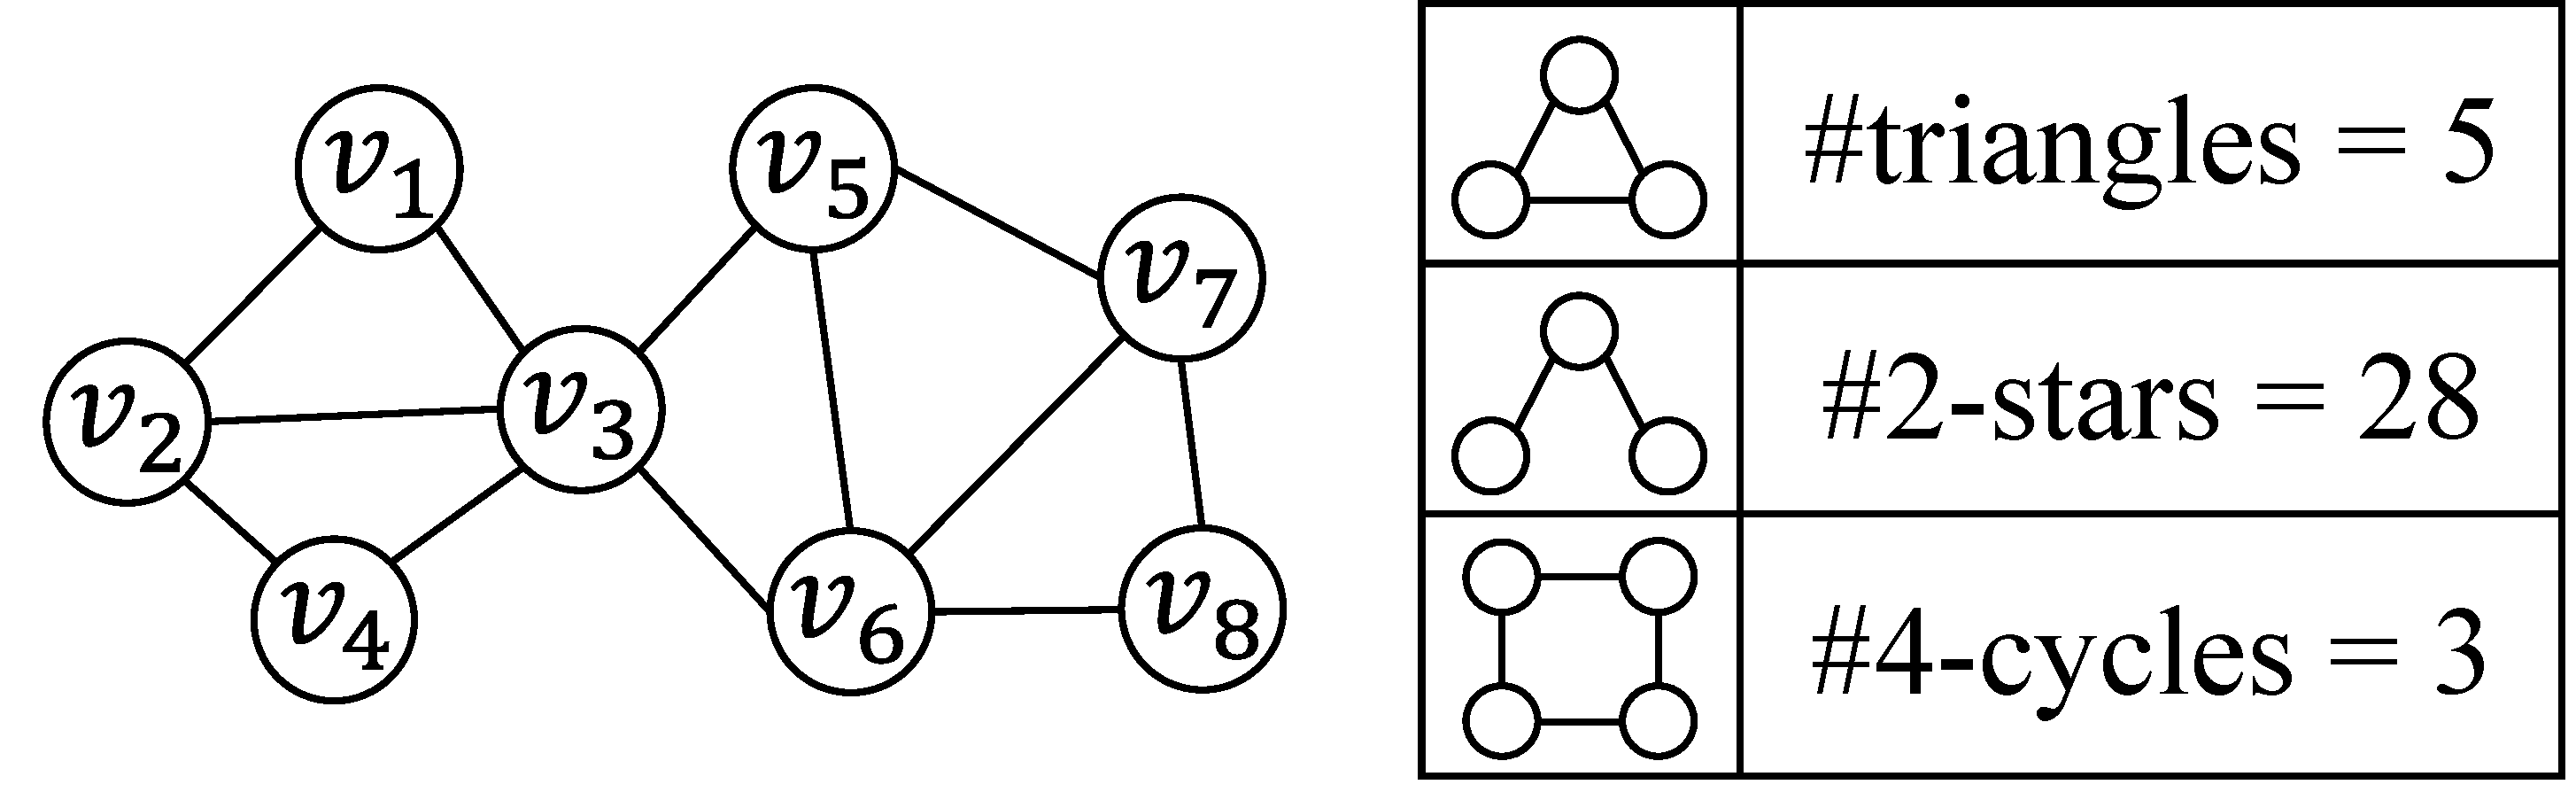
\includegraphics[width=0.65\linewidth]{fig/subgraphs.pdf}
  
  \caption{Examples of subgraph counts.
  }
  \label{chap3-fig:subgraphs}
\end{figure}

DP (Differential Privacy) \cite{Dwork_ICALP06,DP} -- the gold standard of privacy notions -- has been widely used to strongly protect edges in graph data \cite{Day_SIGMOD16,Ding_TKDE21,Hay_ICDM09,Imola_USENIX21,Imola_USENIX22,Karwa_PVLDB11,Kasiviswanathan_TCC13,qin2017generating,Sun_CCS19,Ye_ICDE20,Ye_TKDE21}. 
% DP strongly protects user privacy when a parameter (privacy budget) $\epsilon$ is small and is known as the gold standard of privacy notions. 
% against adversaries with any background knowledge. 
In particular, recent studies 
\cite{Imola_USENIX21,Imola_USENIX22,qin2017generating,Ye_ICDE20,Ye_TKDE21} 
% \cite{Imola_USENIX21,Imola_USENIX22,Ye_ICDE20,Ye_TKDE21} 
have applied LDP (Local DP) \cite{Kasiviswanathan_FOCS08} to 
graph data. 
% subgraph counting. 
% where each user has 
%subgraph counting. 
In the graph LDP model, each user obfuscates her neighbor list (friends list) by herself and sends the obfuscated neighbor list to a data collector. 
Then, the data collector estimates graph statistics, such as subgraph counts. 
Compared to central DP where a central server has personal data of all users (i.e., the entire graph), LDP does not have a risk that all personal data are leaked from the server by 
% illegal access 
cyberattacks 
\cite{Henriquez_breach2021} or insider attacks \cite{Kohen_insider_threats}. 
Moreover, LDP can be applied to decentralized social networks \cite{Paul_CN14,Salve_CSR18} (e.g., diaspora* \cite{Diaspora}, Mastodon \cite{Mastodon}) where no server can access the entire graph; e.g., 
the entire graph is distributed across many servers, or no server has any original edges. 
It is reported in \cite{Imola_USENIX21} that $k$-star counts can be accurately estimated in this model. 

However, it is much more challenging to accurately count more complicated subgraphs such as triangles and 4-cycles under LDP. 
The root cause of this is its local property -- a user cannot see edges between others. 
% For example, user $v_3$ knows that there are ten $2$-stars of which she is a center. 
% However, $v_3$ cannot count triangles or 4-cycles including $v_3$, as she cannot see edges between others, e.g., $(v_1,v_2)$ and $(v_2,v_4)$. 
For example, user $v_1$ cannot count triangles or 4-cycles including $v_1$, as she cannot see edges between others, e.g., $(v_2,v_3)$, $(v_2,v_4)$, and $(v_3,v_4)$. 
Therefore, the existing algorithms \cite{Imola_USENIX21,Imola_USENIX22,Ye_ICDE20,Ye_TKDE21} 
obfuscate 
each bit of the neighbor list 
% each user's edges 
rather than the subgraph count by 
% apply 
% Warner's 
the RR (Randomized Response) \cite{Warner_JASA65}, which randomly flips 0/1. 
% with some probability, 
% to each bit of the neighbor list. 
As a result, their algorithms suffer from extremely large estimation errors because it makes all edges noisy. 
% any triangle or 4-cycle. 
% To address this issue, 
Some studies \cite{Imola_USENIX21,Imola_USENIX22} 
significantly improve the accuracy by introducing 
% introduce 
an additional round of interaction between users and the data collector. 
% Their algorithms publish the noisy graph at the first round to enable each user to count her triangles such that only one edge is noisy at the second round. 
% In their algorithms, the data collector publishes the noisy graph at the first round. 
% Specifically, they propose triangle algorithms that publish the noisy graph at the first round 
% so that each user can count her triangles at the second round. 
% Then, at the second round, each user can count her triangles such that only one edge is noisy. 
% because she knows two edges connected to her. 
% Therefore, the accuracy is significantly improved. 
% Thus, the two-rounds algorithms significantly reduce the estimation error. 
However, multi-round interaction may be impractical in many applications, as it requires a lot of user effort and synchronization; 
in  \cite{Imola_USENIX21,Imola_USENIX22}, every user must respond twice, and the data collector must wait for responses from all users 
in each round. 
% to publish the noisy graph. 

In this work, we focus on a \textbf{one-round} of interaction between users and the data collector and propose accurate subgraph counting algorithms by introducing a recently studied privacy model: the \textit{shuffle model} \cite{Erlingsson_SODA19,Feldman_FOCS21}. 
% The shuffle model introduces an intermediate server called the shuffler. 
In the shuffle model, each user sends her (encrypted) obfuscated data to an intermediate server called the shuffler. 
Then, the shuffler randomly shuffles the obfuscated data of all users and sends the shuffled data to the data collector (who decrypts them). 
% It has been proven that 
The shuffling amplifies DP guarantees of the obfuscated data under the assumption that the shuffler and the data collector do not collude with each other. 
Specifically, it is known that DP strongly protects user privacy when a parameter (a.k.a. privacy budget) $\epsilon$ is small, e.g., $\epsilon \leq 1$ \cite{DP_Li}. 
The shuffling significantly reduces $\epsilon$ and therefore significantly improves utility at the same value of $\epsilon$. 
To date, the shuffle model has been successfully applied to tabular data \cite{Meehan_ICLR22,Wang_PVLDB20} and 
% image data 
gradients \cite{Girgis_AISTATS21,Liu_AAAI21} in federated learning. 
We 
%make the first attempt (to our knowledge) to apply the shuffle model to subgraph counting. 
apply the shuffle model to graph data to accurately count subgraphs within one round. 
%one-round subgraph counting to provide a small estimation error. 

% However, it is very challenging to apply the shuffle model to subgraph counting because 
The main challenge in subgraph counting in the shuffle model is that each user's neighbor list is \textit{high-dimensional data}, i.e., $n$-dim binary string where $n$ is the number of users. 
% we cannot use the entire neighbor list as input data. 
Consequently, applying the RR to each bit of the neighbor list, as in the existing work \cite{Imola_USENIX21,Imola_USENIX22,Ye_ICDE20,Ye_TKDE21}, results in an extremely large privacy budget $\epsilon$ even after applying the shuffling (see Section~\ref{chap3-sub:technical} for more details). 

We address this issue by introducing a new, basic technique called \textit{wedge shuffling}. 
In graphs, a wedge between $v_i$ and $v_j$ is defined by a 2-hop path with endpoints $v_i$ and $v_j$. 
% Our wedge shuffle technique obfuscates a wedge (2-hop path) between a specific user-pair. 
% rather than the entire neighbor list. 
For example, in Figure~\ref{chap3-fig:subgraphs}, 
there are two wedges between $v_2$ and $v_3$: $v_2$-$v_1$-$v_3$ and $v_2$-$v_4$-$v_3$. 
In other words, users $v_1$ and $v_4$ have a wedge between $v_2$ and $v_3$, whereas $v_5, \ldots, v_8$ do not. 
Each user obfuscates such wedge information by the RR, and the shuffler randomly shuffles them. 
Because the wedge information (i.e., whether there is a wedge between a specific user-pair) 
is \textit{one-dimensional binary data}, it can be sent with small noise and small $\epsilon$. 
In addition, the wedge is the main component of several subgraphs, such as triangles, 4-cycles, and 3-hop paths \cite{Sun_CCS19}. 
Since the wedge has little noise, we can accurately count these subgraphs based on wedge shuffling. 

We apply wedge shuffling to triangle and 4-cycle counting tasks with several additional techniques. 
For triangles, we first 
%consider a problem of counting 
propose an algorithm that counts triangles involving the user-pair at the endpoints of the wedges by locally sending an edge between the user-pair to the data collector. 
% along with shuffled wedges. 
% to count triangles including the user-pair. 
Then we propose an algorithm to count triangles in the entire graph by sampling disjoint user-pairs, which share no common users (i.e., 
no user falls in two pairs). 
We also propose a technique to reduce the variance of the estimate by ignoring sparse user-pairs, where either of the two users has a very small degree. 
For 4-cycles, we propose an algorithm to calculate an unbiased estimate of the 4-cycle count from that of the wedge count via bias correction. 

% We propose triangle and 4-cycle counting algorithms based on our wedge shuffle technique and show upper bounds on the estimation error for our algorithms. 
We provide upper bounds on the estimation error for our triangle and 4-cycles counting algorithms. 
Through comprehensive evaluation, we show that 
% it is possible to accurately estimate 
our algorithms 
accurately estimate these subgraph counts within one round under the shuffle model. 
% to triangles and 4-cycles. 
% with some additional techniques. 
% Our experimental results show that 

% \begin{itemize}
%     \item shuffle model for graphs?
%     \item define graph shuffle model
%     \item problem: high dim data
%     \item counting triangles/4-cycles
%     \item our approach: dim reduction by wedges
% \end{itemize}


\smallskip
\noindent{\textbf{Our Contributions.}}~~Our contributions are as follows: 
\begin{itemize}
    \item We propose a wedge shuffle technique to enable privacy amplification 
    %in subgraph counting. 
    of graph data. 
    To our knowledge, we are the first to shuffle graph data (see Section~\ref{chap3-sec:related} for more details). 
    %apply the shuffle model to graph data. 
    \item We propose one-round triangle and 4-cycle counting algorithms 
    %with theoretical performance guarantees 
    based on our wedge shuffle technique. 
    %apply wedge shuffling to triangles and 4-cycles. 
    For triangles, we propose three additional techniques: sending local edges, sampling disjoint user-pairs, and variance reduction by ignoring sparse user-pairs. 
    For 4-cycles, we propose a bias correction technique. 
    We show upper bounds on the estimation error for each algorithm. 
    \item We evaluate our algorithms using two real graph datasets. 
    Our experimental results show that our one-round shuffle algorithms 
    significantly outperform one-round local algorithms in terms of accuracy 
    %dramatically the estimation error of the one-round local algorithms 
    and achieve a small estimation error (relative error $\ll 1$) with a reasonable privacy budget, e.g., smaller than $1$ in edge DP. 
\end{itemize}
In \conference{the full version of this paper \cite{Imola_CCSFull22}}\arxiv{Appendix~\ref{chap3-sec:cluster}}, we show that our triangle algorithm is also useful for accurately estimating the clustering coefficient within one round. 
% we can also accurately estimate the clustering coefficient within one round by using our triangle algorithm. 
We can use our algorithms to analyze the clustering tendency or the effectiveness of friend suggestions in decentralized social networks by introducing a shuffler. 
We implemented our algorithms in C/C++. 
Our code is available on GitHub \cite{SubgraphShuffle}. 
The proofs of all statements in the main body are given in \conference{\cite{Imola_CCSFull22}}\arxiv{Appendices~\ref{chap3-sec:triangle_proof} and \ref{chap3-sec:4cycle_proof}}. 
